\documentclass[10pt,aspectratio=169]{beamer}

\usepackage{kotex}
\setsanshangulfont[AutoFakeBold=2,AutoFakeSlant=.2]{Noto Sans CJK KR}
\usepackage{amsmath,amssymb,mathtools}
\usepackage{graphicx}
\usepackage{booktabs}
\usepackage{xurl}
\usepackage{tikz}
\usepackage{hyperref}

\graphicspath{{figures_ko/}{figures/}}
\definecolor{navy}{HTML}{142B44}
\definecolor{blue}{HTML}{2166AC}
\definecolor{teal}{HTML}{1B8A8F}
\definecolor{orange}{HTML}{E67E22}
\definecolor{red}{HTML}{B2182B}
\definecolor{cream}{HTML}{F7F4ED}
\definecolor{lightblue}{HTML}{EAF2F8}
\definecolor{graytext}{HTML}{4B5563}

\setbeamercolor{normal text}{fg=navy,bg=white}
\setbeamercolor{structure}{fg=blue}
\setbeamercolor{frametitle}{fg=white,bg=navy}
\setbeamercolor{title}{fg=white}
\setbeamercolor{subtitle}{fg=white!78}
\setbeamercolor{author}{fg=white}
\setbeamercolor{institute}{fg=white!82}
\setbeamercolor{date}{fg=white!75}
\setbeamercolor{block title}{fg=white,bg=blue}
\setbeamercolor{block body}{fg=navy,bg=lightblue}
\setbeamercolor{alerted text}{fg=red}
\setbeamerfont{frametitle}{series=\bfseries,size=\large}
\setbeamerfont{title}{series=\bfseries,size=\LARGE}
\setbeamertemplate{navigation symbols}{}
\setbeamertemplate{bibliography item}[text]
\setbeamertemplate{itemize item}{\color{teal}$\blacktriangleright$}
\setbeamertemplate{itemize subitem}{\color{orange}$\bullet$}
\setbeamertemplate{footline}{%
  \leavevmode\hbox{%
  \begin{beamercolorbox}[wd=.82\paperwidth,ht=2.7ex,dp=1.2ex,leftskip=1.2em]{author in head/foot}%
  \color{graytext}\scriptsize 얇은 껍질 근사의 유효성과 힘비 대리지표
  \end{beamercolorbox}%
  \begin{beamercolorbox}[wd=.18\paperwidth,ht=2.7ex,dp=1.2ex,rightskip=1.2em plus1fil]{author in head/foot}%
  \color{graytext}\scriptsize\insertframenumber/\inserttotalframenumber
  \end{beamercolorbox}}}
\hypersetup{colorlinks=true,urlcolor=orange}

\newcommand{\qnum}{Q_{\mathrm{num}}}
\newcommand{\qlr}{Q_{\mathrm{LR}}}
\newcommand{\qsurf}{Q_{\mathrm{surf}}}
\newcommand{\qctr}{Q_{\mathrm{ctr}}}
\newcommand{\qms}{Q_{\mathrm{MS}}}
\newcommand{\qas}{Q_{\mathrm{AS}}}

\title{카멜레온 얇은 껍질 근사는\\언제 실패하는가?}
\subtitle{수치 스칼라 전하 정확도와 힘비 임계값 대리지표 지도}
\author{이동규}
\institute{서울대학교 물리천문학부}
\date{고전역학 기말 프로젝트 --- 독립 개정 연구, 2026년 7월 10일}

\begin{document}

\begin{frame}[plain]
 \begin{tikzpicture}[remember picture,overlay]
  \fill[navy] (current page.south west) rectangle (current page.north east);
  \fill[teal,opacity=.20] (current page.south west) -- ++(7.0,0) -- ++(-2.0,9.0) -- cycle;
  \fill[orange,opacity=.18] (current page.north east) -- ++(-5.5,0) -- ++(2.0,-9.0) -- cycle;
 \end{tikzpicture}
 \vspace{0.8cm}
 \titlepage
 \vfill
 \centering\scriptsize\color{white!80}
 \href{https://github.com/Lasqui-Ponto/Mechanics_Term_Project/tree/agent/improve-chameleon-project/Thin_Shell_Study}{GitHub의 Thin\_Shell\_Study}
\end{frame}

\begin{frame}{1. 연구 공백은 또 하나의 시연이 아니라 오차 추정이다}
 \begin{columns}[T,onlytextwidth]
  \begin{column}{0.47\textwidth}
   \begin{block}{알려진 근사식}
    \[
      Q_{\rm KW}=\min\!\left(3\frac{\Delta R}{R},1\right)
    \]
    하나의 수가 비선형 구면 경계값 문제를 대신한다.
   \end{block}
   \vspace{0.15cm}
   \begin{itemize}
    \item 빠르고 물리적으로 투명하다
    \item 얇은 껍질과 무거운 핵을 가정해 유도된다
    \item 대개 정확도 추정 없이 사용된다
   \end{itemize}
  \end{column}
  \begin{column}{0.49\textwidth}
   \begin{block}{연구 질문}
    \centering\large
    힘비 임계값의 \alert{위}와 \alert{아래}를 가르기에\\
    이 근사식은 충분히 정확한가?
   \end{block}
   \vspace{0.18cm}
   \begin{enumerate}
    \item 완전한 비선형 장을 푼다.
    \item 수치 스칼라 전하를 측정한다.
    \item 근사 오차를 지도화한다.
    \item 오차를 대리 판정 경계까지 전파한다.
   \end{enumerate}
  \end{column}
 \end{columns}
 \vfill
 \centering\color{graytext}\small
 독자적 기여: 최초의 얇은 껍질 계산이 아니라 \textbf{정확도와 관측 가능성을 연결하는 것}.
\end{frame}

\begin{frame}{2. 균일 구는 두 개의 독립적인 제어변수를 남긴다}
 \begin{columns}[T,onlytextwidth]
  \begin{column}{0.54\textwidth}
   \small
   \[
    V(\phi)=\frac{\Lambda^5}{\phi},\qquad
    \nabla^2\phi=-\frac{\Lambda^5}{\phi^2}+\frac{\rho}{M_c}
   \]
   \[
    x=\frac rR,\quad u=\frac{\phi}{\phi_\infty},\quad
    \delta=\frac{\rho_c}{\rho_\infty},\quad \mu=m_\infty R
   \]
   \begin{block}{완전한 비선형 BVP ($n=1$, 약결합 극한)}
    \[
     u''+\frac{2}{x}u'=\frac{\mu^2}{2}
     \left[\widetilde\rho(x)-u^{-2}\right]
    \]
    \[
     u'(0)=0,\qquad u(\infty)=1
    \]
   \end{block}
  \end{column}
  \begin{column}{0.42\textwidth}
   \vspace{0.15cm}
   \begin{block}{추가 입력이 아닌 진단량}
    \[
     \epsilon=\frac{2(1-\delta^{-1/2})}
     {\mu^2\delta}
    \]
    \[
     m_cR=\mu\delta^{3/4}
    \]
   \end{block}
   \begin{itemize}
    \item $\epsilon\ll1$: 기하학적으로 얇은 껍질
    \item $m_cR\gg1$: 핵이 유효 퍼텐셜의 최소에 도달
    \item $\mu\ll1$: 원천이 외부 작용 범위보다 작음
   \end{itemize}
  \end{column}
 \end{columns}
 \vfill
 \scriptsize\color{graytext}
 완전한 지수 결합의 무차원화에는 $D=\phi_\infty/M_c$도 포함된다. 주 스캔은 표준 근사식과 같은 $D\to0$ 극한을 명시적으로 취한다.
\end{frame}

\begin{frame}{3. 장거리 법칙만으로 유한 범위의 전하 위치는 정해지지 않는다}
 \small
 \begin{columns}[T,onlytextwidth]
  \begin{column}{0.31\textwidth}
   \begin{block}{장거리 법칙}
    \[
      \qlr=\min(3\epsilon,1),\quad \mu\ll1
    \]
    선형 껍질 질량에 경험적 상한을 둔다.
   \end{block}
  \end{column}
  \begin{column}{0.31\textwidth}
   \begin{block}{두 가지 단순 연장}
    \[
      \qsurf=\qlr
    \]
    \[
      \qctr=e^{-\mu}\qlr
    \]
    유효 전하를 표면 또는 중심에 둔다.
   \end{block}
  \end{column}
  \begin{column}{0.34\textwidth}
   \begin{block}{활성 껍질 적분}
    \[
     g(z)=z\cosh z-\sinh z
    \]
    \[
     \qas=\frac{3e^{-\mu}}{\mu^3}
     [g(\mu)-g(\mu q)]
    \]
    활성화된 반지름 껍질에 유카와 가중치를 준다.
   \end{block}
  \end{column}
 \end{columns}
 \vspace{0.3cm}
 \begin{block}{관례에 관한 주의}
  \centering
  표면 기준 $Q$에는 $e^{-\mu}$가 들어간다. 중심 기준 균일 구의 형상인자
  $3[\mu\cosh\mu-\sinh\mu]/\mu^3$는 1보다 크다.
 \end{block}
 \centering\color{graytext}
 $\qas$는 여기서 구성하고 검증한 식이며, 문헌상 최초의 공식이라고 주장하지 않는다.
\end{frame}

\begin{frame}{4. 외부 꼬리에서 수치 스칼라 전하를 측정한다}
 \begin{columns}[T,onlytextwidth]
  \begin{column}{0.50\textwidth}
   \begin{block}{스칼라 전하의 정의}
    \[
     u=1-s\qnum\frac{e^{-\mu(x-1)}}{x},
     \qquad s=\frac{\mu^2\delta}{6}
    \]
   \end{block}
   \begin{align*}
    Q_A(x)&=\frac{x(1-u)e^{\mu(x-1)}}{s},\\
    Q_\nabla(x)&=\frac{x^2u'e^{\mu(x-1)}}{s(1+\mu x)}.
   \end{align*}
   두 추정량의 일치는 계산에 내장된 진단 기준이다.
  \end{column}
  \begin{column}{0.46\textwidth}
   \begin{itemize}
    \item 불연속 밀도 경계의 정확한 처리: 두 콜로케이션 영역
    \item 규칙적인 중심 조건과 유카와 Robin 외부 경계
    \item 전하로 스케일한 변수 $x(u-1)=sv$
    \item 어려운 전이점에서는 양의 로그장 표현 사용
    \item 적응형 4차 콜로케이션법(SciPy \texttt{solve\_bvp})
   \end{itemize}
   \vspace{0.2cm}
   \begin{block}{매개변수 스캔}
    \centering
    $25\times29=725$개 점\\
    $10^2\leq\delta\leq10^5$\\
    $10^{-3}\leq\mu\leq0.3$, $x_{\max}=160$
   \end{block}
  \end{column}
 \end{columns}
 \vfill
 \centering\bfseries 725개 매개변수 점이 모두 수렴했다.
\end{frame}

\begin{frame}{5. 검증: 해석적 극한, 수렴성, 독립 추정량}
 \centering
 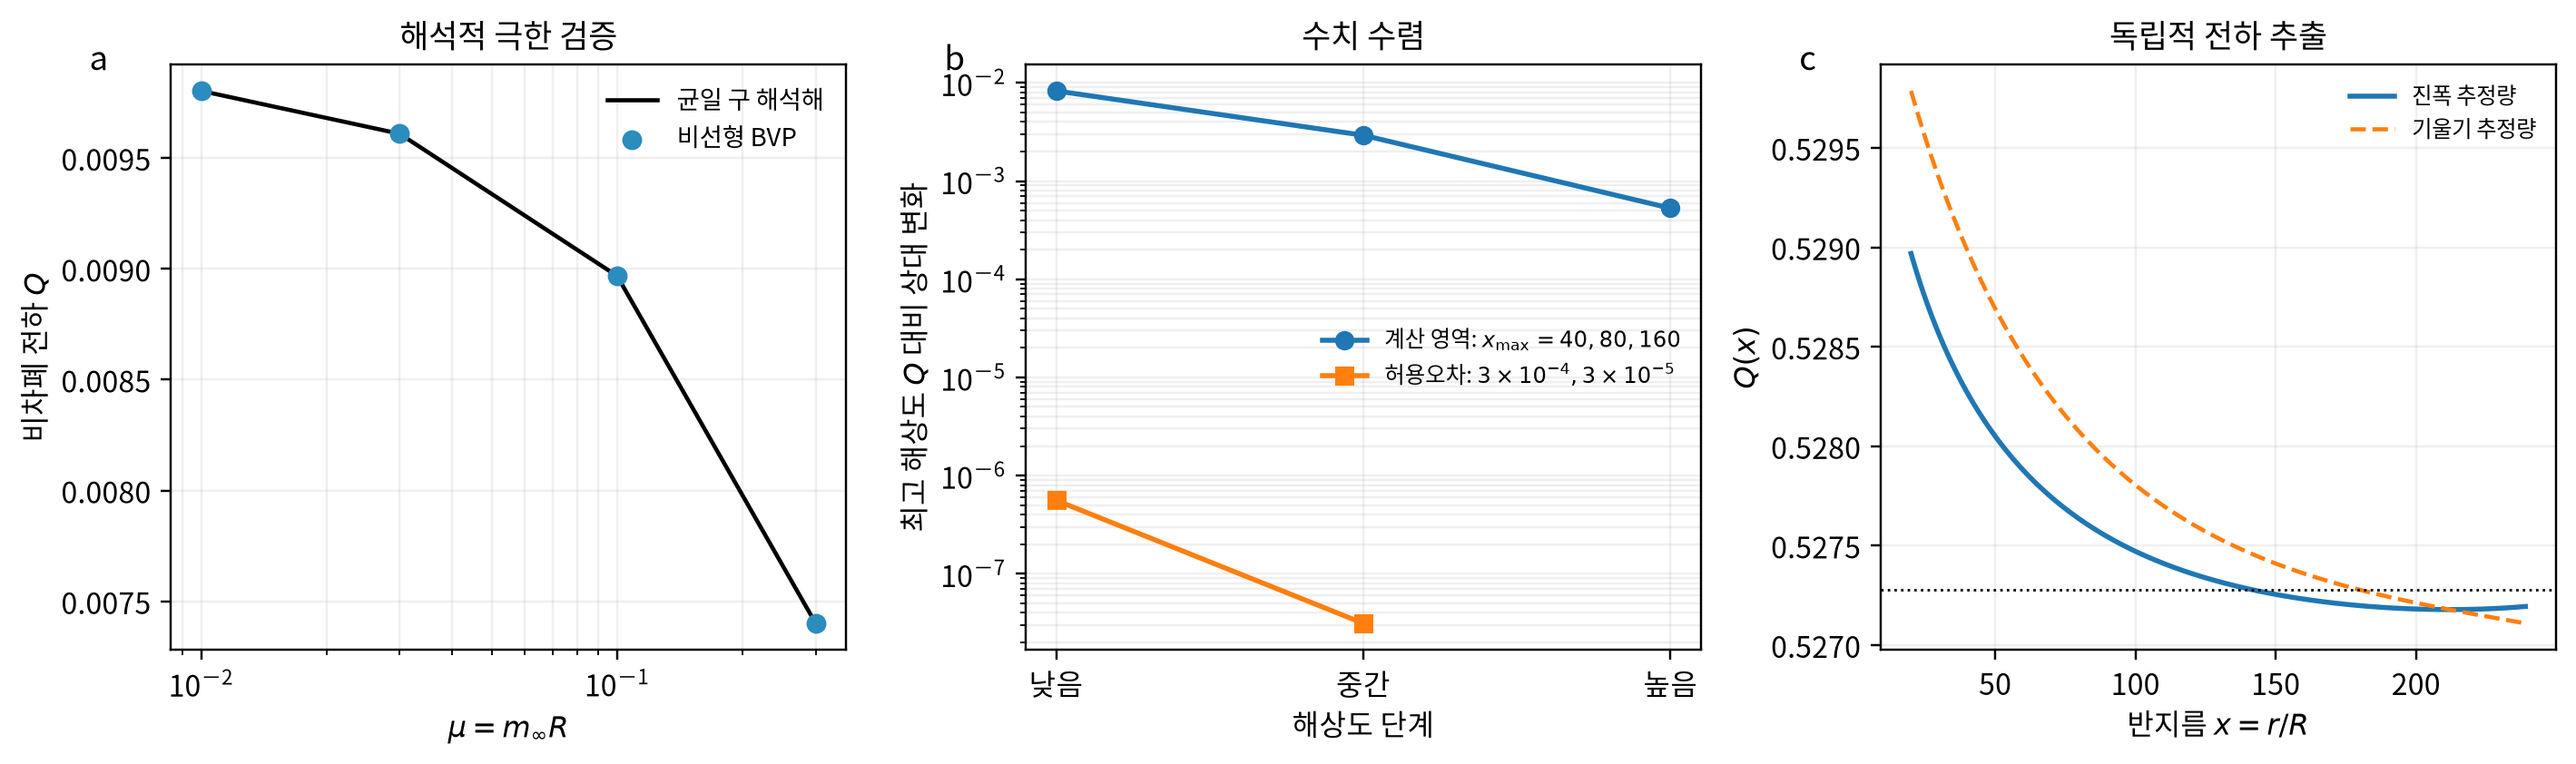
\includegraphics[width=0.96\textwidth]{verification.png}
 \vspace{-0.1cm}
 \begin{columns}[T,onlytextwidth]
  \begin{column}{0.33\textwidth}\centering\scriptsize
   약한 원천의 해석해 오차\\\textbf{최대 $2.8\times10^{-5}$}
  \end{column}
  \begin{column}{0.33\textwidth}\centering\scriptsize
   $x_{\max}=160\to240$ 변화\\\textbf{0.0528\%}
  \end{column}
  \begin{column}{0.33\textwidth}\centering\scriptsize
   전체 지도에서 추정량 불일치\\\textbf{최대 0.0481\%}
  \end{column}
 \end{columns}
 \vspace{0.18cm}
 \centering\small
 층화 표본 14개 점의 $160\to240$ 검증: 전하 변화 \textbf{최대 0.0560\%},
 10\% 정확도 판정 변화 \textbf{0개}.
\end{frame}

\begin{frame}{6. BVP는 비차폐·전이·차폐 영역을 모두 푼다}
 \centering
 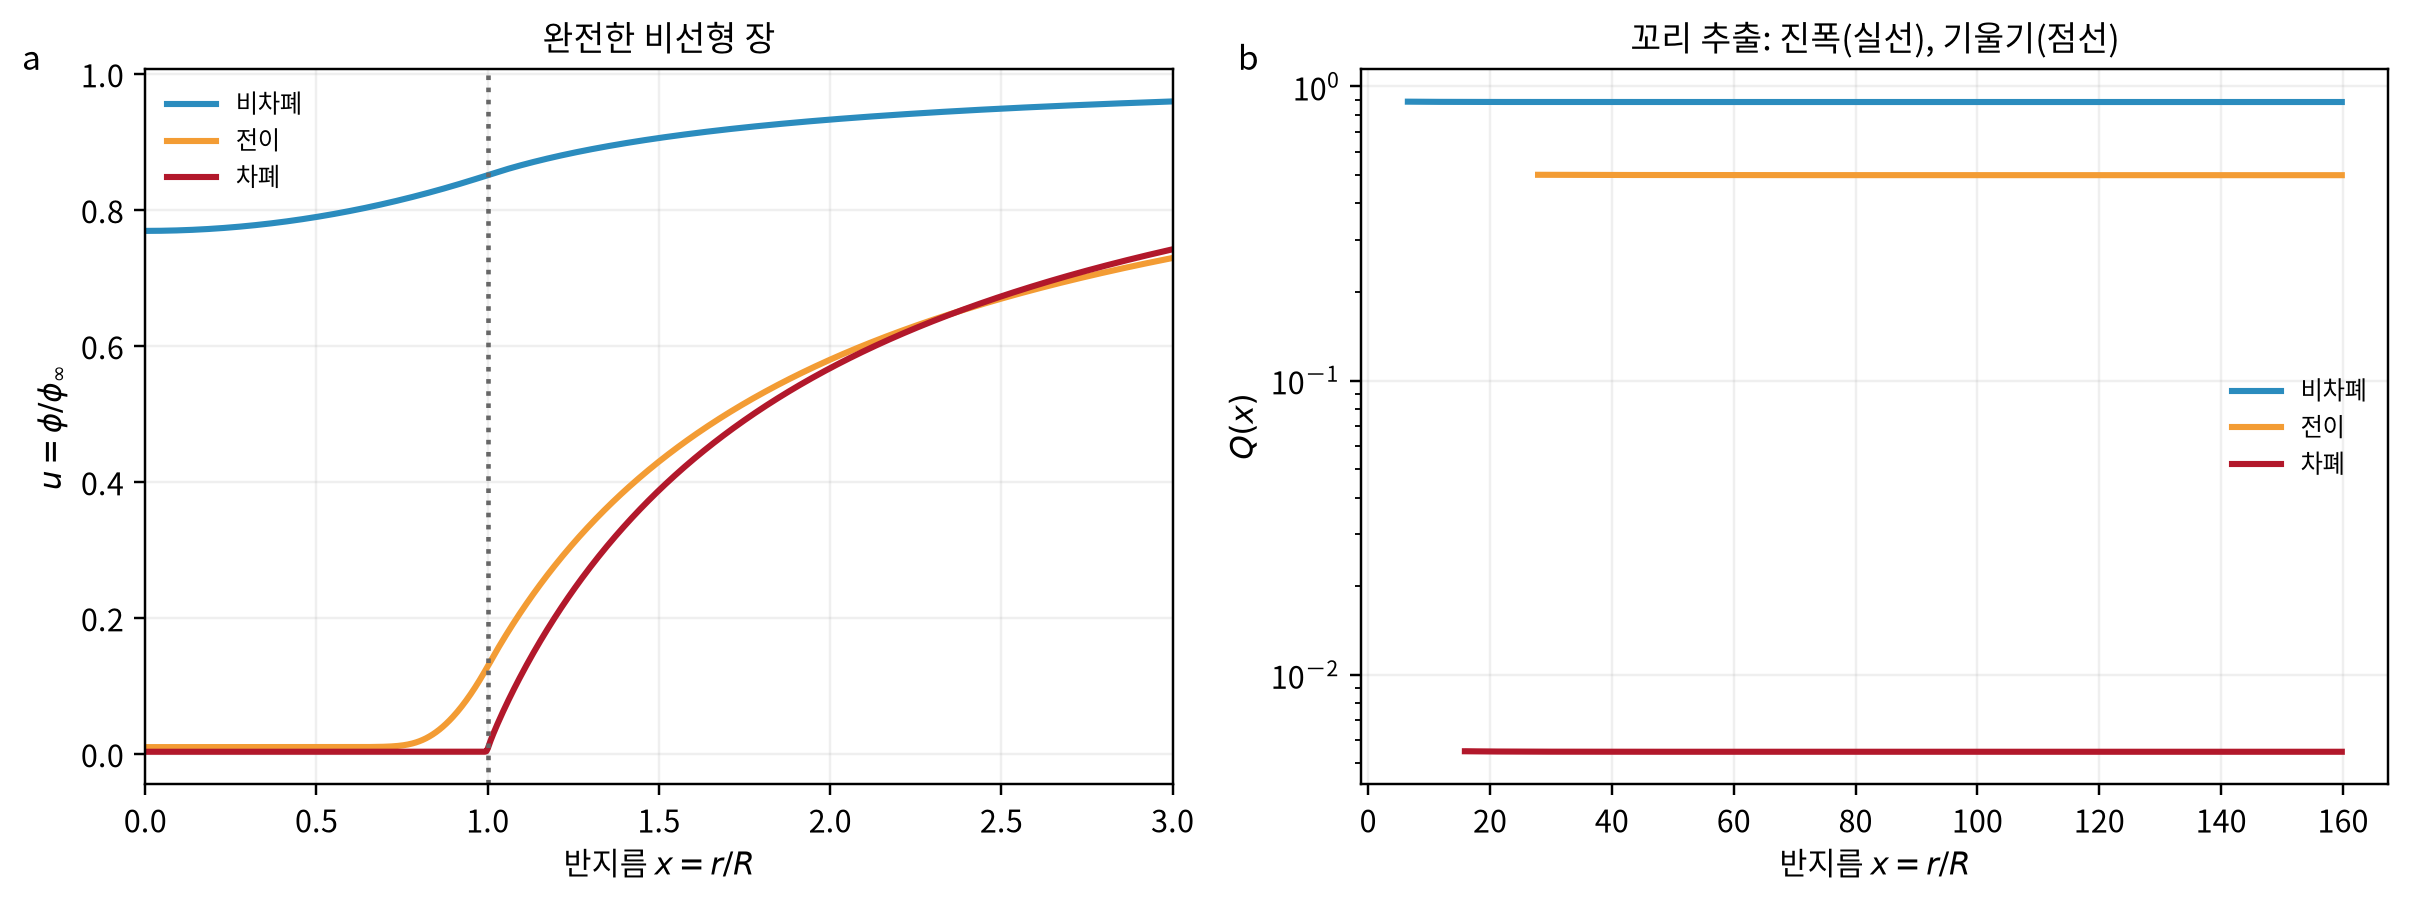
\includegraphics[width=0.93\textwidth]{profiles_and_charge_extraction.png}
 \vspace{0.02cm}
 \parbox{0.95\textwidth}{\centering\scriptsize
 $Q_{\rm num}=0.885$(비차폐), $0.499$(전이), $5.47\times10^{-3}$(차폐).\\[3pt]
 전하의 평탄부는 완전한 수치해의 출력이며, 얇은 껍질을 미리 가정하지 않았다.}
\end{frame}

\begin{frame}{7. 핵심 결과: 유한 범위 연장은 유일하지 않다}
 \centering
 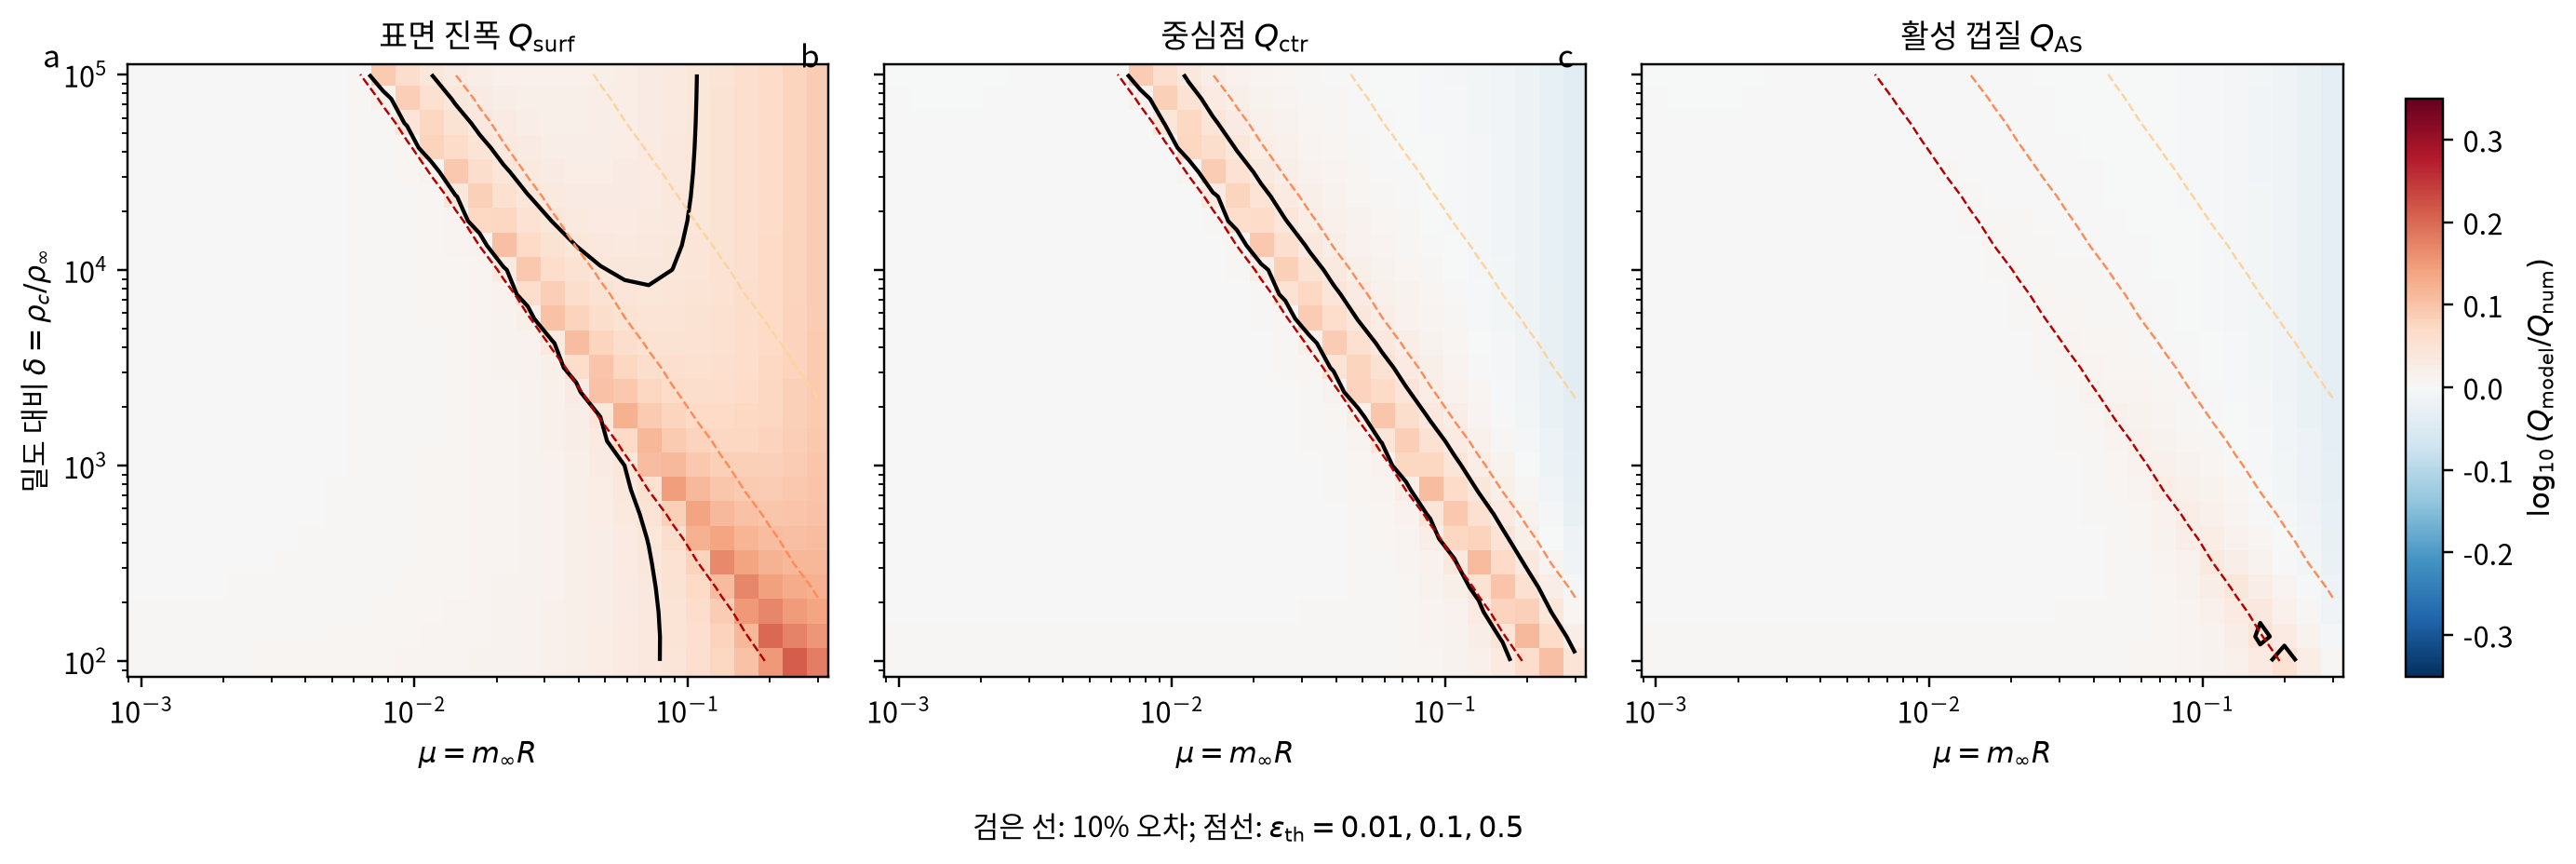
\includegraphics[width=0.97\textwidth]{accuracy_atlas.png}
 \vspace{-0.05cm}
 \scriptsize
 빨강 = 과대 예측, 검은 선 = 10\% 오차 경계, 점선 = 일정한 $\epsilon$.\\
 \alert{표면과 중심 연장은 서로 다르며, 활성 껍질 적분이 수치 경향 대부분을 재현한다.}
\end{frame}

\begin{frame}{8. 활성 껍질 적분이 수치 경향 대부분을 재현한다}
 \begin{columns}[T,onlytextwidth]
  \begin{column}{0.54\textwidth}
   \centering
   \setlength{\tabcolsep}{4pt}
   \begin{tabular}{lrrr}
    \toprule
     & 중앙값 & 최댓값 & $<10\%$ \\
    \midrule
    표면 껍질 & 2.78\% & 62.6\% & 68.8\% \\
    중심점 & 0.566\% & 30.1\% & 91.3\% \\
    \color{blue}활성 껍질 & \color{blue}0.391\% & \color{blue}13.1\% & \color{blue}99.7\% \\
    \bottomrule
   \end{tabular}
   \vspace{0.35cm}
   \begin{block}{장거리 근사의 10\% 정확도에 대한 검증된 조건}
    \[
      \boxed{\epsilon<0.1,\quad m_cR>10,\quad m_\infty R<0.035}
    \]
    지도 17/17개 점과 별도 중간점 12/12개가 통과했다.
   \end{block}
  \end{column}
  \begin{column}{0.42\textwidth}
   \textbf{두 가지 교훈}
   \begin{enumerate}
    \item $3\epsilon$은 껍질 두께의 1차 근사에 불과하다.
    \item 유한 범위에는 전하의 반지름 위치 모형이 필요하다.
   \end{enumerate}
   \vspace{0.25cm}
   \begin{alertblock}{적용 범위}
    ``99.7\%''는 이 $n=1$ 구면 모형과 로그 격자에 대한 결과다.
    모든 카멜레온 퍼텐셜과 기하에 대한 증명은 아니다.
   \end{alertblock}
  \end{column}
 \end{columns}
\end{frame}

\begin{frame}{9. 힘비 대리지표는 장치의 도달범위가 아니다}
 \begin{columns}[T,onlytextwidth]
  \begin{column}{0.52\textwidth}
   \begin{block}{구형 원천 외부에서}
    \[
     \alpha_5\equiv\left|\frac{a_5}{a_N}\right|
     =2\beta^2Q_sQ_t(1+\mu x_p)e^{-\mu(x_p-1)}
    \]
   \end{block}
   주 지도: $\beta=1$, $Q_t=1$, $x_p=1.5$.
   \vspace{0.25cm}
   \[
     \alpha_\star=10^{-2}
   \]
   이는 \textbf{예시적인 무차원 임계값}이다. 유한 범위 연장의 모호성이
   대리 판정을 바꾸는지 확인하기 위해 선택했다.
  \end{column}
  \begin{column}{0.44\textwidth}
   \begin{block}{구분해야 할 세 가지 진술}
    \begin{itemize}
     \item $\alpha_5$: 물리적 신호의 힘비
     \item $\mathcal R=|a_5|/a_{\rm lim}$: 과거 무검출 결과의 도달범위
     \item $\mathcal D=|\Delta a_5|/\sigma_a$: 미래 신호대잡음비 대리지표
    \end{itemize}
   \end{block}
   원자는 $Q_t\simeq1$일 수 있지만 벌크 탐침은 차폐될 수 있다.
   그러나 장치마다 잡음이 다르므로 스칼라 전하만으로 성능을 순위화할 수 없다.
  \end{column}
 \end{columns}
 \vfill
 \centering\color{graytext}\small
 원천의 물리적 스케일과 검출기 잡음을 지정하지 않았으므로, 민감도 곡선이나 배제 곡선이 아니다.
\end{frame}

\begin{frame}{10. 유한 범위 연장 선택이 힘비 대리지표 임계값을 바꾼다}
 \centering
 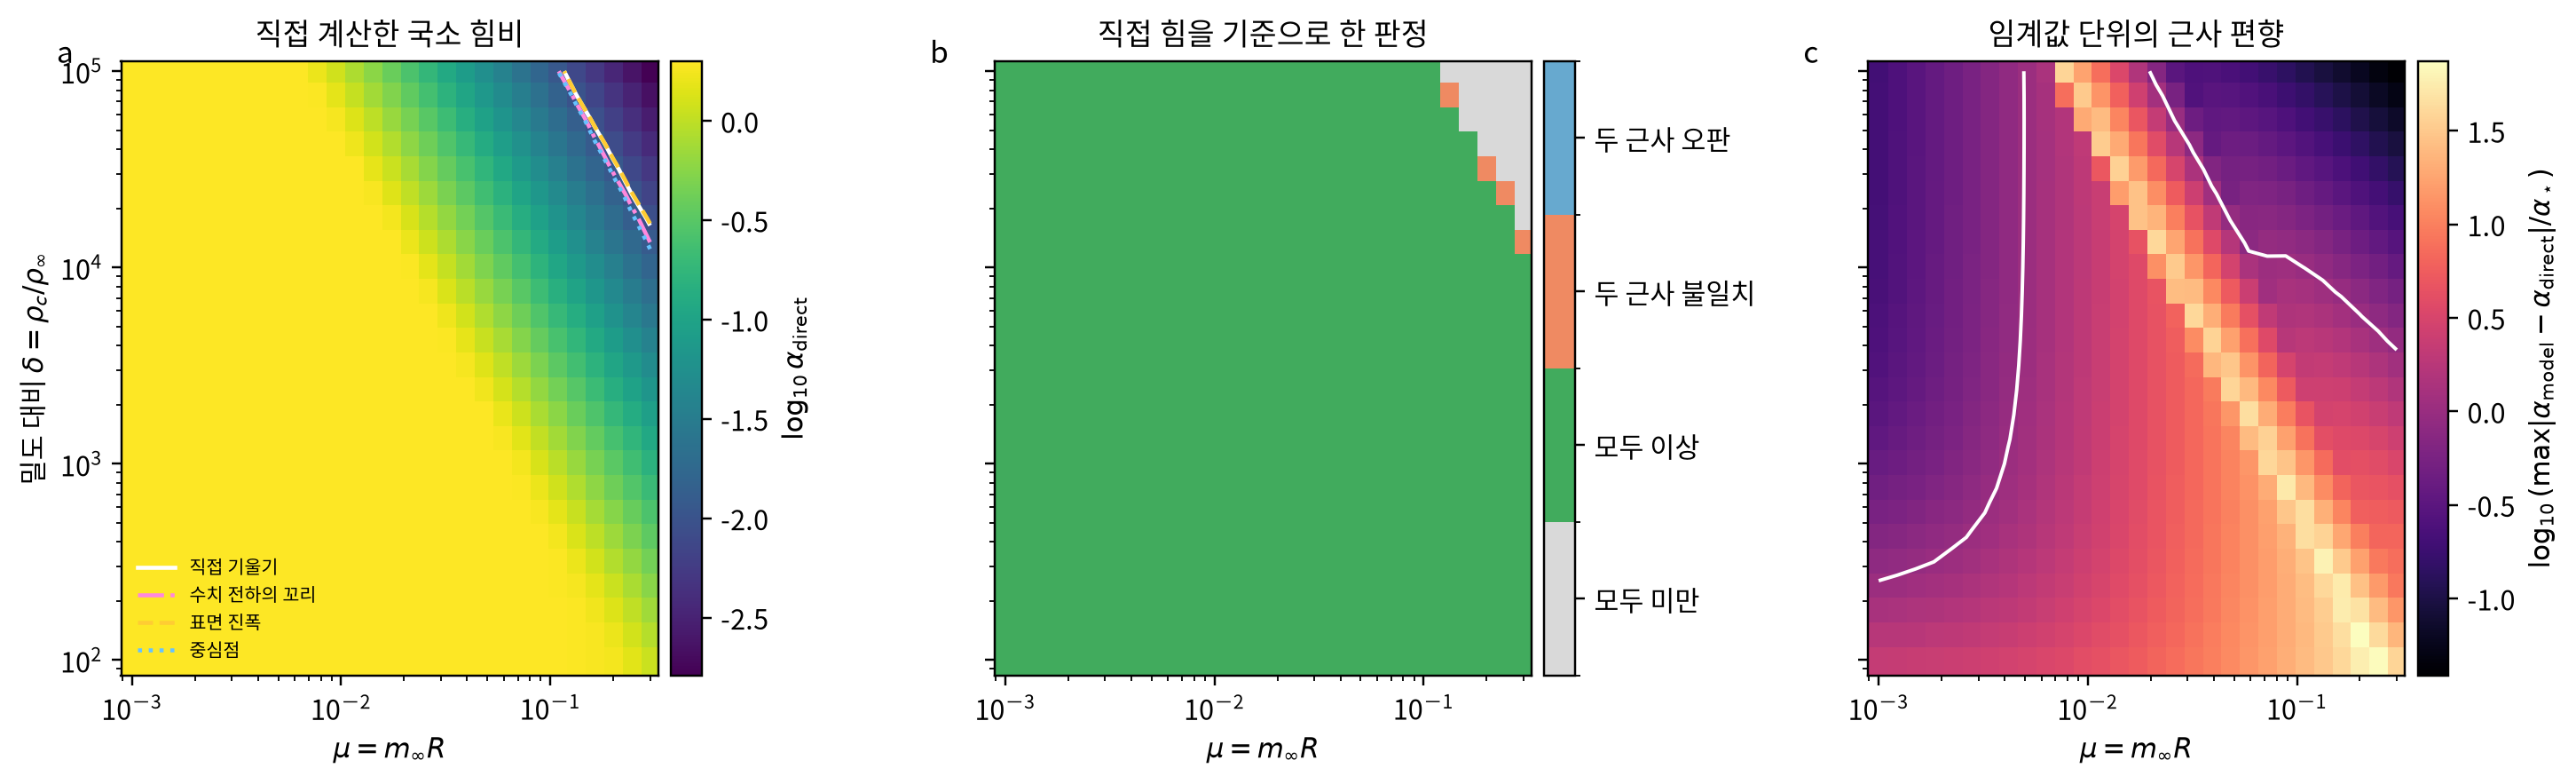
\includegraphics[width=0.97\textwidth]{detectability_map.png}
 \vspace{-0.05cm}
 \begin{columns}[T,onlytextwidth]
  \begin{column}{0.33\textwidth}\centering\scriptsize
   연장 선택에 민감한 점\\\textbf{$\alpha_\star=10^{-2}$에서 725개 중 4개}
  \end{column}
  \begin{column}{0.33\textwidth}\centering\scriptsize
   등고선 이동의 중앙값\\\textbf{표면 0.032 dex / 중심 0.0066 dex}
  \end{column}
  \begin{column}{0.33\textwidth}\centering\scriptsize
   관례에 무관한 불일치\\\textbf{0개: 수치해는 한 연장과 일치}
  \end{column}
 \end{columns}
\end{frame}

\begin{frame}{11. 이 결과가 뜻하는 것과 뜻하지 않는 것}
 \begin{columns}[T,onlytextwidth]
  \begin{column}{0.48\textwidth}
   \begin{block}{정당화할 수 있는 기여}
    \begin{itemize}
     \item 구면 전이 영역의 체계적 오차 지도
     \item 검증된 수치 스칼라 전하 추출
     \item 활성 껍질 유한 범위 가설의 수치 검증
     \item 연장 선택에 따른 임계값 모호성 지도
     \item 재현 가능한 코드, 데이터, 테스트
    \end{itemize}
   \end{block}
  \end{column}
  \begin{column}{0.48\textwidth}
   \begin{alertblock}{주장하지 않는 것}
    \begin{itemize}
     \item 제5힘의 검출
     \item 새로운 물리적 $(\Lambda,M_c)$ 배제 영역
     \item 챔버나 비구형 원천에서의 유효성
     \item $Q_{\rm AS}$의 보편적 정확도나 문헌상 우선권
     \item 기본 암흑에너지 모형의 부활
    \end{itemize}
   \end{alertblock}
  \end{column}
 \end{columns}
 \vspace{0.3cm}
 \small
 챔버 벽과 3차원 기하는 실험실 힘을 바꿀 수 있으며, 기존 수치 연구에서는
 장치별 보정이 수십 퍼센트에 이른다. 2022년 부유형 힘 센서 실험은 조사한 매개변수
 영역에서 우주론적으로 유효한 기본 카멜레온 모형을 배제했다고 보고했다.
 여기서는 이 모형을 근사 제어를 연구하는 비선형 역학 실험실로 사용한다.
\end{frame}

\begin{frame}{12. 결론: 유한 범위 연장, 반지름 구조, 하나의 판정 기준}
 \begin{columns}[T,onlytextwidth]
  \begin{column}{0.61\textwidth}
   \begin{enumerate}
    \item \textbf{68.8\% 대 91.3\%}: 표면 대 중심 연장의 10\% 이내 비율.
    \item \textbf{62.6\%}: 표면 연장의 최악 과대 예측.
    \item \textbf{99.7\%}: 활성 껍질 적분의 10\% 이내 비율.
   \end{enumerate}
   \vspace{0.25cm}
   \begin{block}{이 스캔에서 얻은 실용적 판정 기준}
    얇은 껍질만으로는 부족하다. 무거운 핵과, 외부 콤프턴 파장보다 작은 원천도 필요하다.
    \[
      \epsilon<0.1,\quad m_cR>10,\quad m_\infty R<0.035.
    \]
   \end{block}
  \end{column}
  \begin{column}{0.35\textwidth}
   \begin{block}{연구의 의미}
    장거리 법칙만으로는 유한 범위의 전하 위치를 고를 수 없다.
    활성 전하의 반지름 분포가 결과를 결정한다.
   \end{block}
   \vspace{0.25cm}
   \centering
   \href{https://github.com/Lasqui-Ponto/Mechanics_Term_Project/tree/agent/improve-chameleon-project/Thin_Shell_Study}{\color{orange}\bfseries 소스, 데이터, 테스트, PDF}\\[5pt]
   \scriptsize
   \texttt{Thin\_Shell\_Study/}
  \end{column}
 \end{columns}
 \vfill
 \centering\Large\bfseries 질문 있습니까?
\end{frame}

\begin{frame}{주요 참고문헌}
 \footnotesize
 \begin{thebibliography}{9}
  \bibitem{KW} J. Khoury and A. Weltman, \emph{Phys. Rev. Lett.} 93, 171104 (2004); \emph{Phys. Rev. D} 69, 044026 (2004).
  \bibitem{TT} T. Tamaki and S. Tsujikawa, \emph{Phys. Rev. D} 78, 084028 (2008).
  \bibitem{Review} C. Burrage and J. Sakstein, \emph{Living Rev. Relativ.} 21, 1 (2018).
  \bibitem{Atom} C. Burrage, E. Copeland, and E. Hinds, \emph{JCAP} 03, 042 (2015).
  \bibitem{Elder} B. Elder et al., \emph{Phys. Rev. D} 94, 044051 (2016).
  \bibitem{Sabulsky} D. Sabulsky et al., \emph{Phys. Rev. Lett.} 123, 061102 (2019).
  \bibitem{Yin} P. Yin et al., \emph{Nature Phys.} 18, 1181--1185 (2022).
 \end{thebibliography}
 \vfill
 \scriptsize
 전체 참고문헌, 유도 과정, 한계, 재현 방법은 보고서에 수록했다.
\end{frame}

\end{document}
